\documentclass[11pt,letterpaper]{article}
\usepackage{lmodern}
\usepackage[T1]{fontenc}
\usepackage{amsmath}
\usepackage{amssymb}
\usepackage{amsfonts}
\usepackage{graphicx}
\usepackage{geometry}
\usepackage{hyperref}

\geometry{top=2.5cm, bottom=2.5cm, left=2.5cm, right=2.5cm}

\title{\textbf{Resumen de la Conferencia de Yuval Peres: Highlights de la Historia de la Probabilidad}}
\author{\textbf{Dylan Gabriel Albor Saucedo} \\ \small Licenciatura en Matemáticas Aplicadas y Computación \\ \small FES Acatlán, UNAM}
\date{}

\begin{document}

\maketitle


A principios del siglo XX, la probabilidad no era tan rigurosa como otras áreas de las matemáticas. En 1900, David Hilbert publicó su famosa lista de problemas y en el \textbf{Sexto Problema} pidió formalizar la física y la probabilidad.

El primer gran paso lo dio Émile Borel en 1909 con los \textbf{números normales}. Un número es normal si sus dígitos aparecen con la misma frecuencia asintótica. Si medimos cuántas veces sale un dígito $D$ en los primeros $n$ decimales de $X$, se debe cumplir:
\begin{equation}
\lim_{n \to \infty} \frac{N_n(D)}{n} = \frac{1}{B}
\end{equation}
Borel demostró que casi cualquier número en el intervalo $[0,1]$ es normal en todas las bases (lo que significa medida de Lebesgue 1). Peres mencionó una frase de Avi Wigderson: sabemos que casi todos los números son normales, pero construir uno solo que lo sea en varias bases a la vez es como ``no poder encontrar paja en un pajar'', un problema abierto muy difícil.

El rigor total llegó en 1933 cuando \textbf{Andréi Kolmogórov} publicó sus axiomas usando la Teoría de la Medida. Creó el espacio $(\Omega, \mathcal{F}, P)$ y aportó herramientas clave como la \textbf{Desigualdad Máxima de Kolmogórov}:
\begin{equation}
P\left( \max_{1 \le k \le n} |S_k| \ge \lambda \right) \le \frac{\text{Var}(S_n)}{\lambda^2}
\end{equation}
Esto permitió avanzar muchísimo en los teoremas de límites y demostrar la Ley Fuerte de los Grandes Números pidiendo solo que el primer momento sea finito.


La probabilidad continuó avanzando al estudiar los procesos a largo plazo. Alexander Khinchin propuso la \textbf{Ley del Logaritmo Iterado} (LIL), que mide qué tan lejos puede llegar una caminata aleatoria:
\begin{equation}
\limsup_{n \to \infty} \frac{S_n}{\sqrt{2n \log \log n}} = 1
\end{equation}
Para demostrarlo, Khinchin usó un truco genial: en lugar de revisar cada paso de tiempo, analizó los puntos de una secuencia exponencial ($n = 2^k$) y luego interpoló, una base clave para las desigualdades de concentración de hoy en día.

En el caso continuo, Norbert Wiener formalizó el \textbf{Movimiento Browniano} en los años 20. Aunque estas curvas son continuas, se demostró que no se pueden diferenciar en ningún punto. Más adelante, Paul Lévy dio otra forma de construirlo refinando trayectorias paso a paso.

Por otro lado, \textbf{George Pólya} estudió las caminatas en rejillas $\mathbb{Z}^d$ y demostró algo muy famoso: una caminata aleatoria simétrica siempre regresa al origen (es recurrente) si estás en 1 o 2 dimensiones. Pero a partir de 3 dimensiones, se pierde (es transitoria). Kakutani lo resumía de forma divertida: \textit{``Un hombre borracho siempre encontrará el camino a su casa, pero un pájaro borracho se perderá para siempre''}.

Una parte central de la clase fue cuando el profesor Peres explicó en el pizarrón la prueba del Teorema del Límite Central (TLC) hecha por \textbf{Lindeberg} en 1922. Es una demostración muy limpia porque no usa funciones características, sino expansiones de Taylor.

Si tenemos variables independientes $X_i$ con media 0, varianza 1 y tercer momento finito, queremos ver que $S_n / \sqrt{n}$ se comporta como una Normal estándar $Z \sim \mathcal{N}(0,1)$. Lindeberg aprovechó que la Normal es estable: si sumas $n$ normales independientes y divides entre $\sqrt{n}$, sigues teniendo una Normal.

La idea es cambiar las variables reales $X_i$ por variables normales $Z_i$ una por una. Para una etapa $k$, definimos una variable intermedia $Y$ con las que ya cambiamos y las que faltan. Evaluamos la diferencia usando Taylor:
\begin{equation}
f\left(Y + \frac{X_k}{\sqrt{n}}\right) = f(Y) + \frac{X_k}{\sqrt{n}}f'(Y) + \frac{X_k^2}{2n}f''(Y) + R_3(X_k)
\end{equation}
Al aplicar la esperanza matemática, como los momentos de $X_k$ y $Z_k$ están emparejados (ambos tienen media 0 y varianza 1), los términos de primer y segundo orden de la expansión se cancelan exactamente:
\begin{equation}
E\left[\frac{X_k}{\sqrt{n}}f'(Y)\right] = 0, \quad E\left[\frac{X_k^2}{2n}f''(Y)\right] = \frac{1}{2n}E[f''(Y)]
\end{equation}
Así que la diferencia en cada paso depende solo del residuo de tercer orden, que es del orden de $\mathcal{O}(n^{-3/2})$. Como hacemos este cambio $n$ veces para completar la suma, el error total acumulado es de $n \times \mathcal{O}(n^{-3/2}) = \mathcal{O}(n^{-1/2})$. Cuando $n \to \infty$, este error se va a cero y queda demostrado el TLC.

A mitad del siglo XX, la probabilidad se cruzó con otras áreas:
\begin{itemize}
\item \textbf{Kiyosi Itô} inventó el \textbf{Cálculo Estocástico} para poder trabajar con funciones del movimiento browniano (que no son diferenciables), creando la famosa Fórmula de Itô.
\item \textbf{Joe Doob} desarrolló las \textbf{Martingalas}, que son como caminatas aleatorias generales pero con propiedades de análisis muy fuertes.
\item \textbf{Hillel Furstenberg} (quien fue el asesor de tesis de Peres) llevó las caminatas aleatorias a grupos matemáticos y estudió el crecimiento de matrices que no conmutan.
\end{itemize}

Al final de la charla, Peres habló de la \textbf{percolación} (redes de nodos conectados al azar). El misterio era saber si los límites de estos modelos discretos tenían \textbf{Invarianza Conforme} al hacer la red infinitamente fina. Stanislav Smirnov logró demostrarlo en 2001 para la rejilla triangular, resolviendo una hipótesis del físico John Cardy y ganando la Medalla Fields en 2010. Esto abrió paso al estudio del SLE (\textit{Schramm-Loewner Evolution}) propuesto por Oded Schramm.

\newpage
\section{Simulaciones Computacionales}
Como parte práctica y siguiendo la historia que contó Peres sobre cómo usaban la computadora en 1991 para revisar las teorías matemáticas, corrí un código para simular estos dos fenómenos.

\space{3.cm}
Simulé una caminata simétrica en $\mathbb{Z}^2$ de $10,000$ pasos (Figura \ref{fig:walk}). Como demostró Pólya, se nota cómo la trayectoria llena mucho el espacio y regresa sobre sus propios pasos de forma constante, lo que visualmente explica por qué la probabilidad de retorno es 1.

\begin{figure}[htbp]
\centering
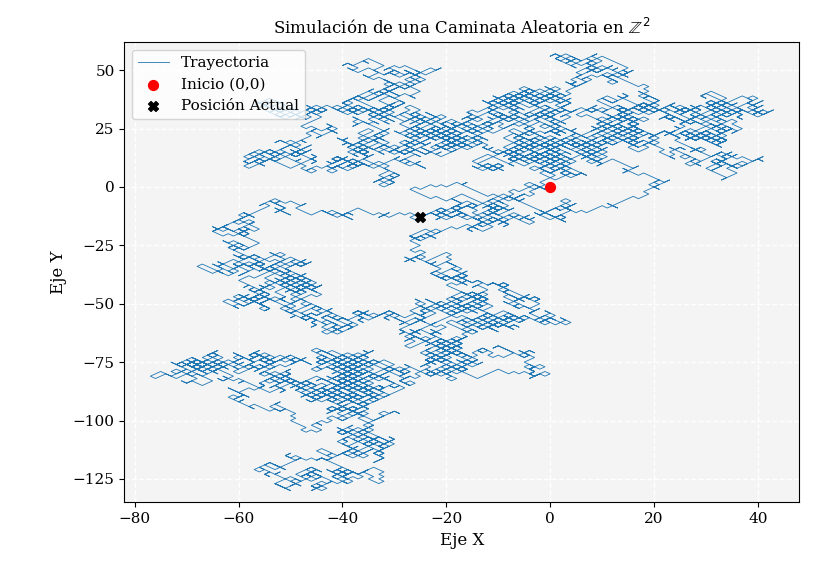
\includegraphics[width=0.52\textwidth]{Figure_1.png}
\caption{Trayectoria de una caminata aleatoria discreta en 2D.}
\label{fig:walk}
\end{figure}

\subsection{Verificación del TLC}
Para ver el TLC al estilo de Lindeberg, tomé $30,000$ muestras que son la suma de 10 variables uniformes independientes (centradas y normalizadas). El histograma de la Figura \ref{fig:clt} muestra cómo, con apenas 10 variables, la distribución empírica se ajusta casi perfecto a la curva de la campana de Gauss teórica.

\begin{figure}[htbp]
\centering
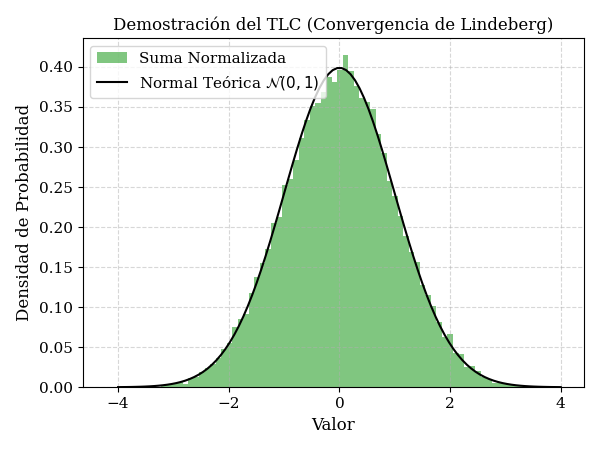
\includegraphics[width=0.52\textwidth]{Figure_2.png}
\caption{Histograma de las sumas simuladas comparado con la curva Normal estándar.}
\label{fig:clt}
\end{figure}

\section{Conclusión}
La plática del profesor Peres muestra de forma muy clara cómo la probabilidad pasó de ser un juego de azar a conectarse con la física cuántica, la geometría y la computación. Hacer simulaciones ayuda mucho a entender el fondo de los teoremas abstractos que vemos en la carrera, dándonos una mejor perspectiva como futuros matemáticos o computólogos.

\end{document}